% A LaTeX template for EXECUTIVE SUMMARY of the MSc Thesis submissions to 
% Politecnico di Milano (PoliMi) - School of Industrial and Information Engineering
%
% P. F. Antonietti, S. Bonetti, A. Gruttadauria, G. Mescolini, A. Zingaro
% e-mail: template-tesi-ingind@polimi.it
%
% Last Revision: October 2021
%
% Copyright 2021 Politecnico di Milano, Italy. Inc. All rights reserved.

\documentclass[11pt,a4paper,twocolumn]{article}

%------------------------------------------------------------------------------
%	REQUIRED PACKAGES AND  CONFIGURATIONS
%------------------------------------------------------------------------------
% PACKAGES FOR TITLES
\usepackage{titlesec}
\usepackage{color}

% PACKAGES FOR LANGUAGE AND FONT
\usepackage[utf8]{inputenc}
\usepackage[english]{babel}
\usepackage[T1]{fontenc} % Font encoding

% PACKAGES FOR IMAGES
\usepackage{graphicx}
\graphicspath{{Images/}} % Path for images' folder
\usepackage{eso-pic} % For the background picture on the title page
\usepackage{subfig} % Numbered and caption subfigures using \subfloat
\usepackage{caption} % Coloured captions
\usepackage{transparent}

% STANDARD MATH PACKAGES
\usepackage{amsmath}
\usepackage{amsthm}
\usepackage{bm}
\usepackage[overload]{empheq}  % For braced-style systems of equations

% PACKAGES FOR TABLES
\usepackage{tabularx}
\usepackage{longtable} % tables that can span several pages
\usepackage{colortbl}

% PACKAGES FOR ALGORITHMS (PSEUDO-CODE)
\usepackage{algorithm}
\usepackage{algorithmic}

% PACKAGES FOR REFERENCES & BIBLIOGRAPHY
\usepackage[colorlinks=true,linkcolor=black,anchorcolor=black,citecolor=black,filecolor=black,menucolor=black,runcolor=black,urlcolor=black]{hyperref} % Adds clickable links at references
\usepackage{cleveref}
\usepackage[square, numbers, sort&compress]{natbib} % Square brackets, citing references with numbers, citations sorted by appearance in the text and compressed
\bibliographystyle{plain} % You may use a different style adapted to your field

% PACKAGES FOR THE APPENDIX
\usepackage{appendix}

% PACKAGES FOR ITEMIZE & ENUMERATES 
\usepackage{enumitem}

% OTHER PACKAGES
\usepackage{amsthm,thmtools,xcolor} % Coloured "Theorem"
\usepackage{comment} % Comment part of code
\usepackage{fancyhdr} % Fancy headers and footers
\usepackage{lipsum} % Insert dummy text
\usepackage{tcolorbox} % Create coloured boxes (e.g. the one for the key-words)
\usepackage{stfloats} % Correct position of the tables
\usepackage{tikz} % For drawing diagrams (needed for tikzpicture environment)

%-------------------------------------------------------------------------
%	NEW COMMANDS DEFINED
%-------------------------------------------------------------------------
% EXAMPLES OF NEW COMMANDS -> here you see how to define new commands
\newcommand{\bea}{\begin{eqnarray}} % Shortcut for equation arrays
\newcommand{\eea}{\end{eqnarray}}
\newcommand{\e}[1]{\times 10^{#1}}  % Powers of 10 notation
\newcommand{\mathbbm}[1]{\text{\usefont{U}{bbm}{m}{n}#1}} % From mathbbm.sty
\newcommand{\pdev}[2]{\frac{\partial#1}{\partial#2}}
% NB: you can also override some existing commands with the keyword \renewcommand

%----------------------------------------------------------------------------
%	ADD YOUR PACKAGES (be careful of package interaction)
%----------------------------------------------------------------------------


%----------------------------------------------------------------------------
%	ADD YOUR DEFINITIONS AND COMMANDS (be careful of existing commands)
%----------------------------------------------------------------------------
\newcommand*{\oldepsilon}{\epsilon}
\renewcommand*{\epsilon}{\varepsilon}
\newcommand*{\oldphi}{\phi}
\renewcommand*{\phi}{\varphi}
\DeclareMathOperator*{\esssup}{ess\,sup}
\DeclareMathOperator*{\argmax}{arg\,max}
\DeclareMathOperator*{\argmin}{arg\,min}


% Do not change Configuration_files/config.tex file unless you really know what you are doing. 
% This file ends the configuration procedures (e.g. customizing commands, definition of new commands)
% Set the geometric layout of the document
\usepackage{geometry}
\geometry{
  top=3cm,
  left = 2.0cm,
  right = 2.0cm,
  bottom=2cm,
  headheight= 2cm,
  headsep= 0cm,
}
\raggedbottom

% Create color bluePoli (-> manuale grafica coordinata:  https://www.polimi.it/fileadmin/user_upload/il_Politecnico/grafica-coordinata/2015_05_11_46xy_manuale_grafica_coordinata.pdf)
\definecolor{bluePoli}{cmyk}{0.4,0.1,0,0.4}

% Custom theorem environments
\declaretheoremstyle[
  shaded={rulecolor=bluePoli!20, rulewidth=1pt, bgcolor=bluePoli!5},
  headfont=\color{bluePoli}\normalfont\bfseries,
  bodyfont=\color{black}\normalfont,
]{colored}

\captionsetup[figure]{labelfont={color=bluePoli}} % Set colour of the captions
\captionsetup[table]{labelfont={color=bluePoli}} % Set colour of the captions
\captionsetup[algorithm]{labelfont={color=bluePoli}} % Set colour of the captions

\theoremstyle{colored}
\newtheorem{theorem}{Theorem}[section]
\newtheorem{proposition}{Proposition}[section]
\newtheorem{definition}{Definition}[section]
\newtheorem*{remark}{Remark}
\newtheorem{lemma}{Lemma}[section]

% Enhances the features of the standard "table" and "tabular" environments.
\newcommand\T{\rule{0pt}{2.6ex}}
\newcommand\B{\rule[-1.2ex]{0pt}{0pt}}

% Algorithm description
\newcounter{algsubstate}
\renewcommand{\thealgsubstate}{\alph{algsubstate}}
\newenvironment{algsubstates}{
    \setcounter{algsubstate}{0}%
    \renewcommand{\STATE}{%
    \stepcounter{algsubstate}%
    \Statex {\small\thealgsubstate:}\space}
    }{}

% Custom theorem environment
\newcolumntype{L}[1]{>{\raggedright\let\newline\\\arraybackslash\hspace{0pt}}m{#1}}
\newcolumntype{C}[1]{>{\centering\let\newline\\\arraybackslash\hspace{0pt}}m{#1}}
\newcolumntype{R}[1]{>{\raggedleft\let\newline\\\arraybackslash\hspace{0pt}}m{#1}}

% Custom itemize environment
\setlist[itemize,1]{label=$\bullet$}
\setlist[itemize,2]{label=$\circ$}
\setlist[itemize,3]{label=$-$}
\setlist{nosep}

% Set separation of columns
\setlength{\columnsep}{30pt}

% Create command for background pic
\newcommand\BackgroundPic{% Adding background picture
	\put(230,358){
		\parbox[b][\paperheight]{\paperwidth}{%
			\vfill
			\centering
			\transparent{0.2}
			
\includegraphics[width=0.8\paperwidth]{raggiera_polimi.eps}%
			\vfill
}}}

% Set indentation
%\setlength\parindent{0pt}

% Custom title commands
\titleformat{\section}
{\color{bluePoli}\normalfont\Large\bfseries}
{\color{bluePoli}\thesection.}{1em}{}
\titlespacing*{\section}
{0pt}{2ex}{1ex}

\titleformat{\subsection}
{\color{bluePoli}\normalfont\large\bfseries}
{\color{bluePoli}\thesubsection.}{1em}{}
\titlespacing*{\subsection}
{0pt}{2ex}{1ex}

\titleformat{\subsubsection}
{\color{bluePoli}\normalfont\normalsize\bfseries}
{\color{bluePoli}\thesubsubsection.}{1em}{}
\titlespacing*{\subsubsection}
{0pt}{2ex}{1ex}

% Custom headers and footers
\pagestyle{fancy}
\fancyhf{}

\fancyfoot{}
\fancyfoot[C]{\thepage} % page
\renewcommand{\headrulewidth}{0mm} % headrule width
\renewcommand{\footrulewidth}{0mm} % footrule width

\makeatletter
\patchcmd{\headrule}{\hrule}{\color{black}\hrule}{}{} % headrule
\patchcmd{\footrule}{\hrule}{\color{black}\hrule}{}{} % footrule
\makeatother

% -> Create the header
\chead[C]{
\centering
\begin{tcolorbox}[arc=0pt, boxrule=0pt, colback=bluePoli!60, width=\textwidth, colupper=white]
    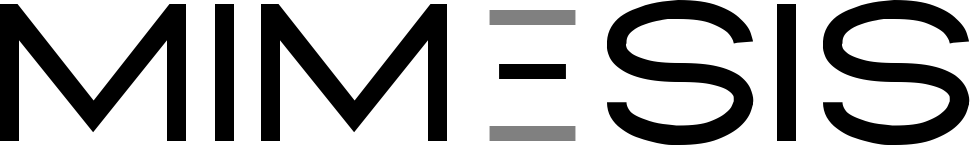
\includegraphics[width=0.2\textwidth]{mimesis.png}
\end{tcolorbox}
}


% Insert here the info that will be displayed into your Title page 
% -> title of your work
\renewcommand{\title}{A Modified Neural Modes Approach for Soft Tissue Simulation}
% -> author name and surname
\renewcommand{\author}{Andrea Bonifacio}
% -> MSc course
\newcommand{\course}{Mathematical Engineering - Ingegneria Matematica}
% -> advisor name and surname
\newcommand{\advisor}{Prof. Stefano Pagani}
% IF AND ONLY IF you need to modify the co-supervisors you also have to modify the file Configuration_files/title_page.tex (ONLY where it is marked)
\newcommand{\firstcoadvisor}{Dr. Stéphane Cotin} % insert if any otherwise comment
%\newcommand{\secondcoadvisor}{Name Surname} % insert if any otherwise comment
% -> academic year
\newcommand{\YEAR}{2024-2025}

%-------------------------------------------------------------------------
%	BEGIN OF YOUR DOCUMENT
%-------------------------------------------------------------------------
\begin{document}

%-----------------------------------------------------------------------------
% TITLE PAGE
%-----------------------------------------------------------------------------
% Do not change Configuration_files/TitlePage.tex (Modify it IF AND ONLY IF you need to add or delete the Co-advisors)
% This file creates the Title Page of the document
% DO NOT REMOVE SPACES BETWEEN LINES!

%\twocolumn[{\begin{@twocolumnfalse}

\AddToShipoutPicture*{\BackgroundPic}

\hspace{-0.6cm}
\includegraphics[width=0.6\textwidth]{logo_polimi_ing_indinf.eps}

\vspace{-1mm}
\fontsize{0.3cm}{0.5cm}\selectfont \bfseries \textsc{\color{bluePoli} Report}\\

\vspace{-0.2cm}
\Large{\textbf{\color{bluePoli}{\title}}}\\

\vspace{-0.2cm}
\fontsize{0.3cm}{0.5cm}\selectfont \bfseries \textsc{\color{bluePoli} \course}\\

\vspace{-0.2cm}
\fontsize{0.3cm}{0.5cm} \selectfont \bfseries Authors: \textsc{\textbf{\author}}\\

%\vspace{-0.4cm}
%\fontsize{0.3cm}{0.5cm}\selectfont \bfseries Advisor: \textsc{\textbf{\advisor}}\\

% if only ONE co-advisor is present:
%\vspace{-0.4cm}
%\fontsize{0.3cm}{0.5cm}\selectfont \bfseries Co-advisor: \textsc{\textbf{\firstcoadvisor}}\\
% if more than one co-advisors are present:
%\vspace{-0.4cm}
%\fontsize{0.3cm}{0.5cm}\selectfont \bfseries Co-advisors: \textsc{\textbf{\firstcoadvisor}}\textsc{\textbf{\secondcoadvisor}}\\

\vspace{-0.4cm}
\fontsize{0.3cm}{0.5cm}\selectfont \bfseries Academic year: \textsc{\textbf{\YEAR}}

\small \normalfont

\vspace{11pt}

\centerline{\rule{1.0\textwidth}{0.4pt}}

%\vspace{15pt}
%\end{@twocolumnfalse}}]

\thispagestyle{plain} % In order to not show the header in the first page


%%%%%%%%%%%%%%%%%%%%%%%%%%%%%%
%%     THESIS MAIN TEXT     %%
%%%%%%%%%%%%%%%%%%%%%%%%%%%%%%

%-----------------------------------------------------------------------------
% INTRODUCTION
%-----------------------------------------------------------------------------

\section{Introduction}
\label{sec:es:introduction}

Numerical simulation is fundamental across science and engineering, enabling the study of complex physical phenomena. In biomedical engineering, accurate simulation of deformable objects, particularly soft tissues, is vital for applications like surgical planning and training. However, traditional methods such as the Finite Element Method (FEM), while accurate, are computationally expensive, making real-time simulation of large, nonlinear deformations challenging.

Model order reduction (ROM) techniques offer a solution by reducing the system's degrees of freedom. Linear ROMs, like those based on modal analysis, provide efficiency but are limited to small deformations and fail to capture the nonlinear behavior of soft tissues.

This thesis addresses the need for efficient and accurate nonlinear simulation by enhancing the ``Neural Modes'' framework \cite{Wang_Du_Coros_Thomaszewski_2024}. This hybrid approach combines the computational speed of linear modal analysis with the function approximation capabilities of deep learning. The core idea is to use linear modes as a basis and train a neural network to learn nonlinear corrections for large deformations and material nonlinearities. By integrating these techniques, the Neural Modes framework aims to overcome the limitations of purely linear ROMs and traditional FEM, enabling accurate and computationally tractable simulations suitable for real-time applications. This work proposes specific modifications to the framework's training and architecture to improve its performance for simulating hyperelastic materials.


\section{Mathematical Framework}
\label{sec:es:mathematical_framework}

Simulating the complex deformation of soft tissues requires a mathematical framework capable of describing their nonlinear mechanical behavior under dynamic conditions. We model the material using the hyperelastic Neo-Hookean constitutive law, which is well-suited for large deformations typical of biological tissues \cite{Ogden_1997}. The material's state is described by its strain-energy density function $\Psi$, from which the first Piola-Kirchhoff stress tensor $\bm{P}$ is derived. For the Neo-Hookean model, the strain-energy density is given by:
\begin{equation}
\begin{split}
        \Psi(\bm{F}) = \frac{\mu}{2} (\text{tr}(\bm{F}^T\bm{F}) - 3 \\- 2\ln(\det(\bm{F}))) + \frac{\lambda}{4} ((\det(\bm{F}))^2\\ - 1 - 2\ln(\det(\bm{F}))),
\end{split}
\label{eq:es:neo_hookean_energy}
\end{equation}
where $\bm{F}$ is the deformation gradient, and $\mu$ and $\lambda$ are Lamé parameters. The stress tensor is $\bm{P} = \partial \Psi / \partial \bm{F}$. For dynamic problems, the equation of motion including inertial forces is:
\begin{equation}
    \begin{cases}
        \rho \frac{\partial^2 \bm{u}}{\partial t^2} - \nabla_X \cdot \bm{P} = \bm{b} \quad \text{in} \quad \Omega, \\
        \bm{u} = \bm{u}_D \quad \text{on} \quad \Gamma_D, \\
        \bm{P} \cdot \bm{N} = \bm{t} \quad \text{on} \quad \Gamma_N,
    \end{cases}
\label{eq:dynamic_problem}
\end{equation}
where $\rho$ is the material density in the reference configuration, $\bm{b}$ is the external body force, $\bm{N}$ is the unit normal to $\Gamma_N$ in the reference configuration, and $\bm{t}$ is the traction applied to the boundary.


To enable efficient simulation of these nonlinear dynamics, we employ linear modal analysis \cite{Pentland_Williams_1989}. This technique linearizes the system around the undeformed state and solves a generalized eigenvalue problem to find the dominant vibration modes:
\begin{equation}
    \bm{K} \bm{\phi}_i = \omega_i^2 \bm{M} \bm{\phi}_i,
\label{eq:es:eigenvalue_problem}
\end{equation}
where $\bm{K}$ is the linear stiffness matrix, $\bm{M}$ is the mass matrix, $\omega_i^2$ are the squared natural frequencies, and $\bm{\phi}_i$ are the mode shapes. The displacement field $\bm{u}$ is approximated as a linear combination of the first $m$ dominant modes:
\begin{equation}
    \bm{u}(\bm{X},t) \approx \sum_{i=1}^{m} q_i(t) \bm{\phi}_i(\bm{X}),
\label{eq:es:modal_decomposition}
\end{equation}
where $q_i(t)$ are the modal coordinates. External forces are projected onto the modal basis to obtain modal forces. While this modal decomposition significantly reduces the problem's dimensionality, the underlying linear assumption limits its accuracy for large, nonlinear deformations.


\section{Methods}
\label{sec:es:methods}

Our approach enhances the ``Neural Modes'' framework, initially proposed by Wang et al. \cite{Wang_Du_Coros_Thomaszewski_2024}, which aims to learn nonlinear deformation subspaces by augmenting linear modal analysis with a neural network. While the original work utilized a self-supervised energy minimization approach, we found this challenging for large deformations due to complex energy landscapes and difficulties in sampling the latent space effectively.

To overcome these limitations, we developed an enhanced framework based on a supervised learning strategy. The core idea remains to represent the total displacement $\bm{u}$ as the sum of a linear modal displacement $\bm{l} = \bm{\Phi} \bm{z}$ and a nonlinear correction $\bm{y}$ predicted by a neural network based on the modal coordinates $\bm{z}$:
\begin{equation}
    \bm{u} = \bm{l} + \bm{y}(\bm{z}).
\label{eq:es:total_displacement_methods}
\end{equation}

The neural network architecture is a deep residual network specifically designed to learn this nonlinear correction. A key design principle is ensuring that the network outputs a zero correction ($\bm{y}=\bm{0}$) when the input modal coordinate vector is zero ($\bm{z}=\bm{0}$), corresponding to the object's rest state. This is achieved by constructing the network entirely from layers that lack bias terms and by initializing the weights of the final output layer to zero. Residual connections are incorporated to facilitate the training of a deep network capable of capturing complex nonlinear relationships.
The internal energy \( E(\bm{u}) \) of the deformed configuration is computed following this equation:


\begin{equation}
    E(\bm{u}) = \int_{\Omega} \Psi(\bm{F}(\bm{u})) \, d\Omega,
\end{equation}
where $\Psi$ is the Neo-Hookean strain energy density function (as defined in Equation \eqref{eq:neo_hookean_energy}). In the context of the loss function, $\bm{u}$ refers to the predicted total displacement $\bm{X} + \bm{l} + \bm{y}$.


The network is trained using a dataset generated from high-fidelity nonlinear FEM simulations. Each data sample consists of a modal coordinate vector $\bm{z}$, the corresponding ground truth full displacement $\bm{u}_{gt}$, and the associated ground truth internal energy $E_{gt}$. The training minimizes a physics-informed loss function, which is a weighted sum of several components:
\begin{itemize}
    \item \textbf{Energy Loss}: Measures the Mean Squared Error between the base-10 logarithms of the predicted internal energy $E(\bm{u})$ and the ground truth energy $E_{gt}$. Using the logarithm helps to handle the wide range of energy values and smooth the loss landscape, improving training stability.
    \begin{equation}
        \mathcal{L}_{energy} = (\log_{10}(E(\bm{u})) - \log_{10}(E_{gt}))^2.
    \end{equation}
    \item \textbf{Displacement Loss}: Computes the Mean Squared Error between the predicted total displacement $\bm{u}$ and the ground truth displacement $\bm{u}_{gt}$.
    \begin{equation}
        \mathcal{L}_{disp} = \|\bm{u} - \bm{u}_{gt}\|^2.
    \end{equation}
    \item \textbf{Orthogonality Loss}: Encourages the learned nonlinear correction $\bm{y}$ to be orthogonal to the linear modal displacement $\bm{l}$.
    \begin{equation}
        \mathcal{L}_{ortho} = (\bm{l}^T \bm{y})^2.
    \end{equation}
        \item \textbf{Boundary Condition Penalty}: enforces the displacement boundary conditions on the deformed configuration. For nodes \( j \) belonging to the set of boundary nodes \( \mathcal{B} \), where the displacement is fixed (e.g., to zero), this loss penalizes deviations from the required displacement. It is defined as the sum of squared displacements at the boundary nodes:
        \begin{equation}
            \mathcal{L}_{BC} = \frac{1}{N} \sum_{i=1}^N \sum_{j \in \mathcal{B}} \|(\bm{u}_i)_j\|^2,
        \end{equation}
        where \( (\bm{u}_i)_j \) is the predicted displacement vector at node \( j \) for the \( i \)-th sample in the batch. This term encourages the network to predict corrections \( \bm{y} \) such that the total displacement \( \bm{u} = \bm{X} + \bm{l} + \bm{y} \) satisfies the fixed boundary conditions.
\end{itemize}
The total loss is a weighted sum of these terms, balancing the importance of displacement accuracy, physical consistency (energy), and the other properties (orthogonality, boundary conditions). This supervised, physics-informed approach allows the network to learn accurate nonlinear corrections and generalize effectively, even with a relatively small dataset, by leveraging the physical information embedded in the loss function.

The conceptual architecture of the Neural Modes framework can be visualized as:

\begin{figure}[H]
    \centering
    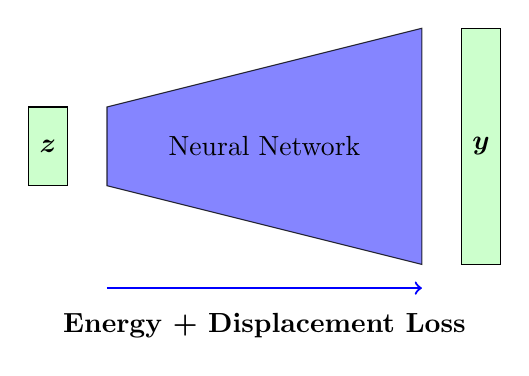
\begin{tikzpicture}
        % Modal coordinate (z)
        \draw[fill=green!20] (-3, 1) rectangle (-2.5,2);
        \node at (-2.75, 1.5) {$\bm{z}$}; % Label inside the rectangle

        % Displacement (u)
        \draw[fill=green!20] (2.5,0) rectangle (3,3);
        \node at (2.75, 1.5) {$\bm{y}$}; % Label inside the rectangle

        % Energy loss transition
        \draw[fill=blue!60,opacity=0.8] (-2,1) -- (2,-0) -- (2,3) -- (-2,2) -- cycle;
        \node at (0,1.5) {Neural Network};
        \node[below] at (0,-0.5) {\textbf{Energy + Displacement Loss}};

        % Energy loss arrow
        \draw[thick,blue,->] (-2,-0.3) -- (2,-0.3);

    \end{tikzpicture}
    \caption{Conceptual illustration of the Neural Modes architecture and training objective.}
    \label{fig:neural_modes_arch_es}
\end{figure}

For generating the training data and validating the framework, we employed a modal force generation approach. This method creates external forces by projecting desired modal amplitudes onto the linear modal basis, ensuring that the generated forces represents realistic deformations following the system's dominant modes. This allows for controlled generation of training data that spans relevant deformation states.

One of the main strenghts of the Neural Modes framework is its ability to perform dynamic simulations. In this context, once we have trained the model, we can use it to predict the system's behavior over time. The model determines the modal coordinates at each time step by solving an optimization problem that minimizes a cost function combining inertial terms and the predicted internal energy of the configuration. This optimization is typically solved using an iterative algorithm like L-BFGS-B. The optimization problem for finding the modal coordinates $\bm{z}_{n+1}$ at time step $n+1$, given states at $n$ and $n-1$, is formulated as:
\begin{equation}
\begin{split}
        \bm{z}_{n+1} = \underset{\bm{z}}{\argmin} \frac{1}{2h^2} \|\bm{n}(\bm{z}) - 2\bm{u}_n + \bm{u}_{n-1}\|_{\bm{M}}^2 \\+ E(\bm{n}(\bm{z})),
\end{split}
    \label{eq:optimization_problem_es}
\end{equation}
where $\bm{n}(\bm{z})$ is the total displacement, $h$ is the time step, $\bm{M}$ is the mass matrix, and $E(\cdot)$ is the total energy of the system. 


\section{Numerical Results}
\label{sec:es:numerical_results}

To evaluate the performance of the enhanced Neural Modes framework, we conducted numerical experiments on a cantilever beam, a standard benchmark for structural mechanics, modeled with Neo-Hookean hyperelastic properties to mimic soft tissue behavior. We also performed tests on a more complex geometry, the Stanford bunny, with similar findings.

\subsection{Optimal Number of Modes}
A crucial initial step was determining the appropriate number of linear modes to use as the basis for the reduced-order model. Using too few modes limits the model's ability to capture complex deformations, while using too many increases computational cost without significant accuracy gains. We analyzed the Root Mean Square Error (RMSE) between the full-order FEM solution and the linear modal approximation as a function of the number of modes. Figure \ref{fig:optimal_number_modes} shows that the error decreases rapidly and then plateaus, indicating that a sufficient basis is achieved with a relatively small number of modes. For our cantilever beam tests, 7 modes were found to be sufficient to capture the dominant deformation patterns relevant to the applied loads.

\begin{figure}[H]
    \centering
    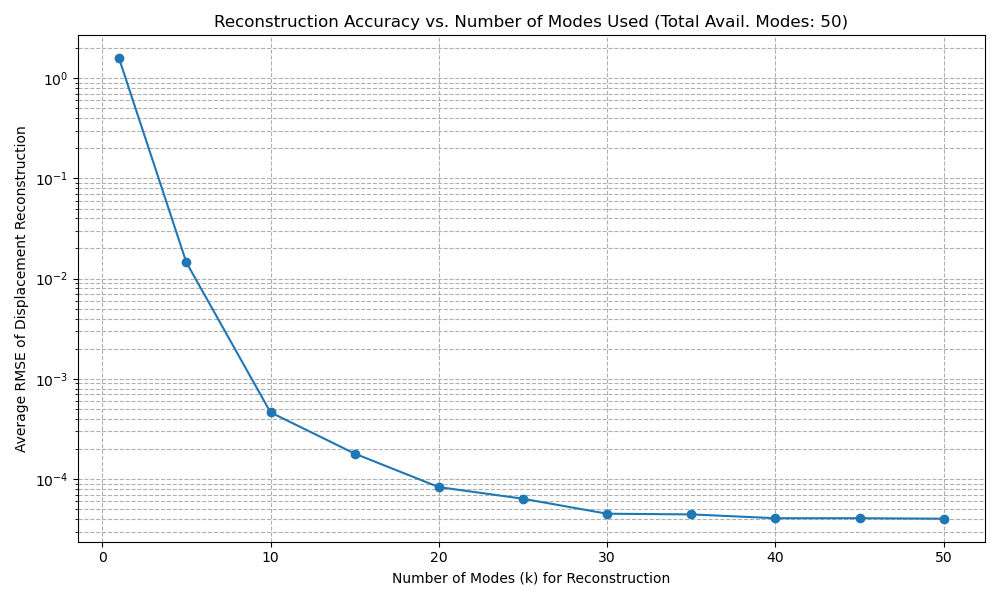
\includegraphics[width=0.45\textwidth]{Images/rmse_vs_modes.png}
    \caption{RMSE of the displacement field vs. number of modes.}
    \label{fig:optimal_number_modes}
\end{figure}

\subsection{Self-Supervised vs. Supervised Training}
We first explored a self-supervised training approach, similar to the original Neural Modes work \cite{Wang_Du_Coros_Thomaszewski_2024}, where the network is trained solely by minimizing the internal energy for randomly sampled modal coefficients. However, validation results showed that this approach yielded subpar performance, achieving accuracy at best comparable to that of the linear modes model, as illustrated by the Mean Squared Error (MSE) comparison in Figure \ref{fig:self_supervised_validation_mse_comparison}. This highlighted the limitations of self-supervised energy minimization for capturing large, nonlinear deformations in our context.

\begin{figure}[H]
    \centering
    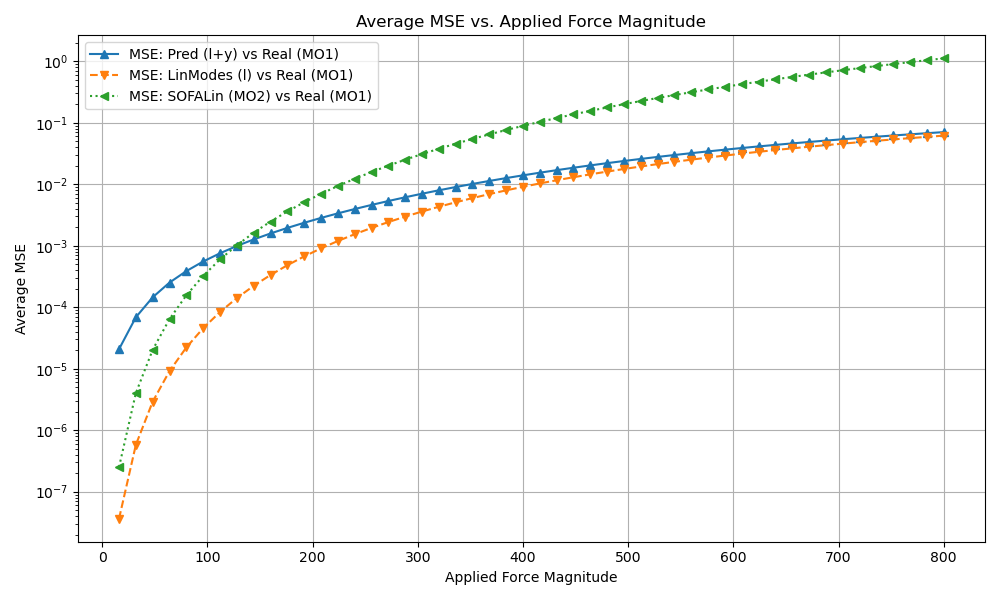
\includegraphics[width=0.45\textwidth]{Images/self_supervised_mse.png}
    \caption{Average MSE comparison for self-supervised training.}
    \label{fig:self_supervised_validation_mse_comparison}
\end{figure}

In contrast, our supervised training strategy, leveraging ground truth data from full nonlinear FEM simulations and a physics-informed loss function, proved significantly more effective.

\subsection{Static Validation}
Static validation on unseen configurations demonstrated the superior accuracy of the supervised Neural Modes model, particularly in the nonlinear deformation regime. Figure \ref{fig:static_mse_comparison} shows the average MSE for the cantilever beam under increasing force, comparing Neural Modes, linear modes, and linear FEM against the nonlinear FEM ground truth. The Neural Modes model significantly outperforms linear methods as nonlinear effects become dominant.

\begin{figure}[H]
    \centering
    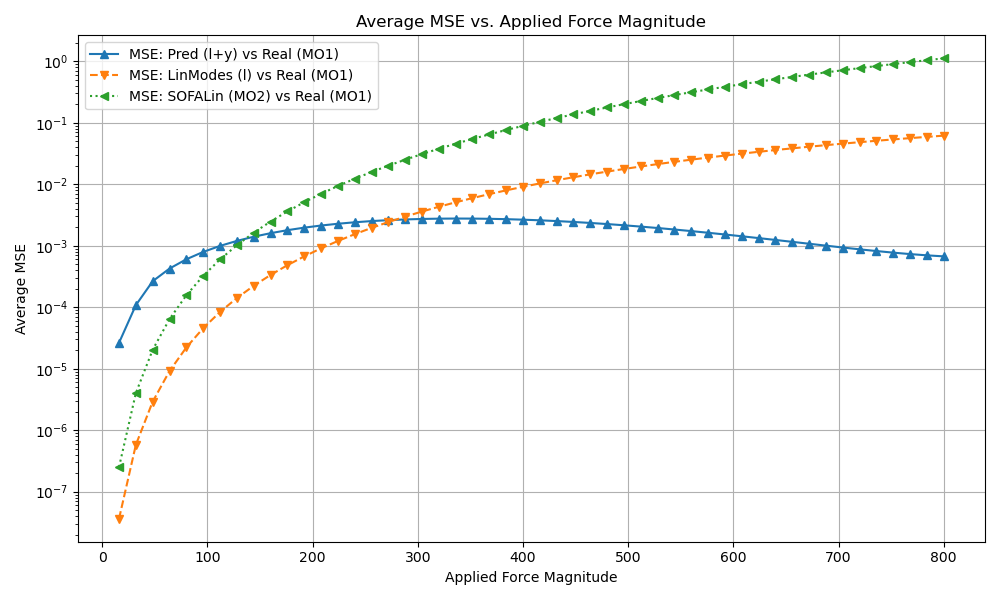
\includegraphics[width=0.45\textwidth]{Images/beam_static_mse.png}
    \caption{Average MSE for static cantilever beam deformation.}
    \label{fig:static_mse_comparison}
\end{figure}

Furthermore, the Neural Modes model maintained physical consistency by predicting internal energy much closer to the ground truth compared to linear methods, which showed significant energy divergence in the nonlinear range (Figure \ref{fig:static_energy_beam}).

\begin{figure}[H]
    \centering
    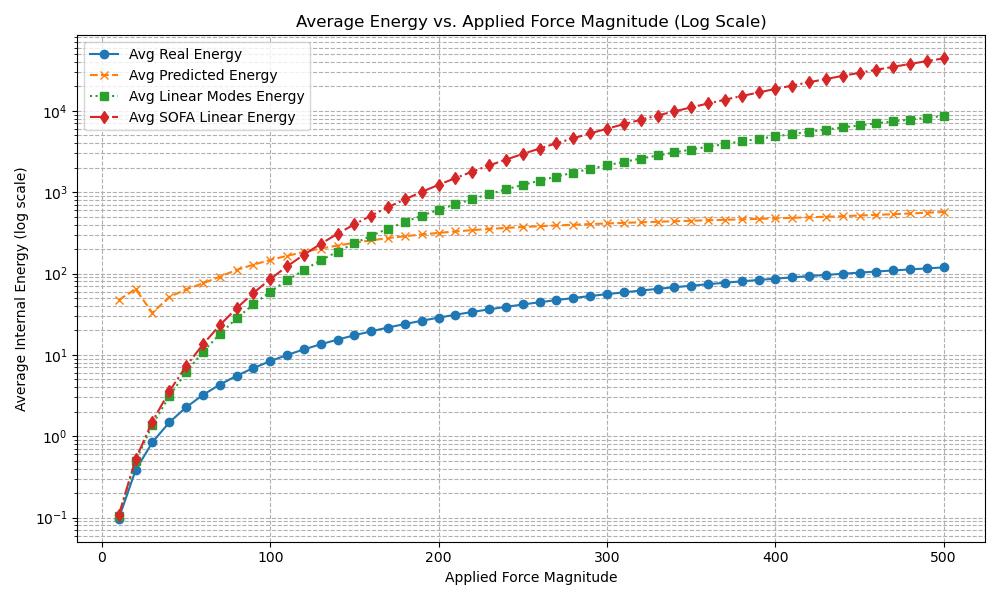
\includegraphics[width=0.45\textwidth]{Images/beam_static_energy.png}
    \caption{Internal energy vs. applied force for static cantilever beam deformation.}
    \label{fig:static_energy_beam}
\end{figure}

Qualitative visual comparisons, such as the one shown in Figure \ref{fig:static_rmse_distribution} for a cantilever beam deformation, further illustrate the Neural Modes model's ability to accurately capture the pronounced bending and complex deformation patterns that linear methods fail to reproduce.

\begin{figure}[H]
    \centering
    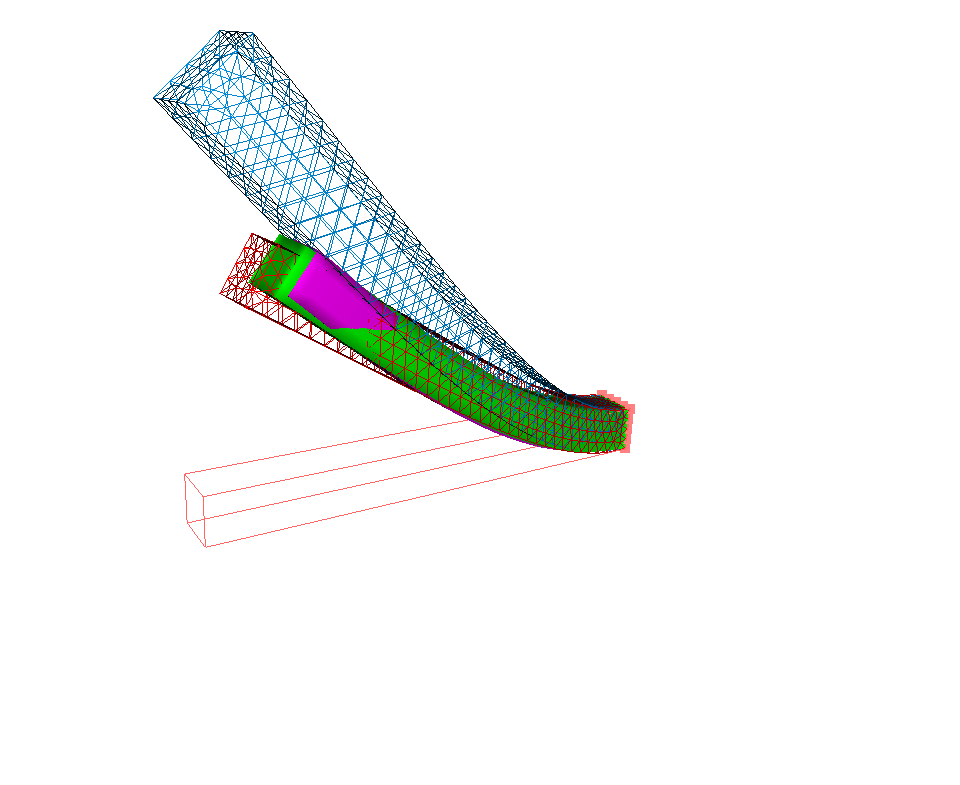
\includegraphics[width=0.45\textwidth]{Images/sofa_example_beam.png}
    \caption{Static deformation example for the cantilever beam. The magenta beam represents the neural modes prediction, while the green beam represents the ground truth. The red wireframe shows the linear modes prediction, and the blue wireframe shows the linear FEM prediction.}
    \label{fig:static_rmse_distribution}
\end{figure}

Similar improvements in accuracy and energy prediction were observed for the Stanford bunny geometry.

\subsection{Dynamic Validation}
Dynamic validation assessed the model's performance over time. We initialized the simulation with the first few time steps from a full nonlinear FEM simulation and then used the Neural Modes model to predict subsequent steps by solving an optimization problem. While the displacement accuracy showed some divergence over extended periods (Figure \ref{fig:dynamic_validation_mse_comparison}), the Neural Modes model maintained internal energy levels significantly closer to the ground truth compared to the linear modes model, which exhibited substantial energy drift (Figure \ref{fig:dynamic_validation_energy_comparison}).

\begin{figure}[H]
    \centering
    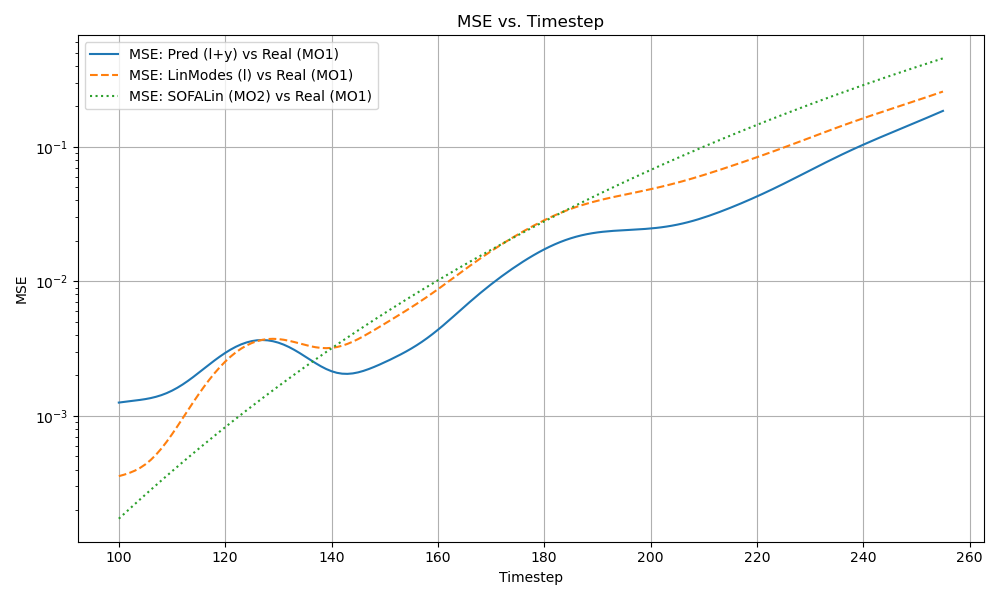
\includegraphics[width=0.45\textwidth]{Images/beam_dynamic_mse.png}
    \caption{MSE over time for dynamic cantilever beam simulation.}
    \label{fig:dynamic_validation_mse_comparison}
\end{figure}

\begin{figure}[htb]
    \centering
    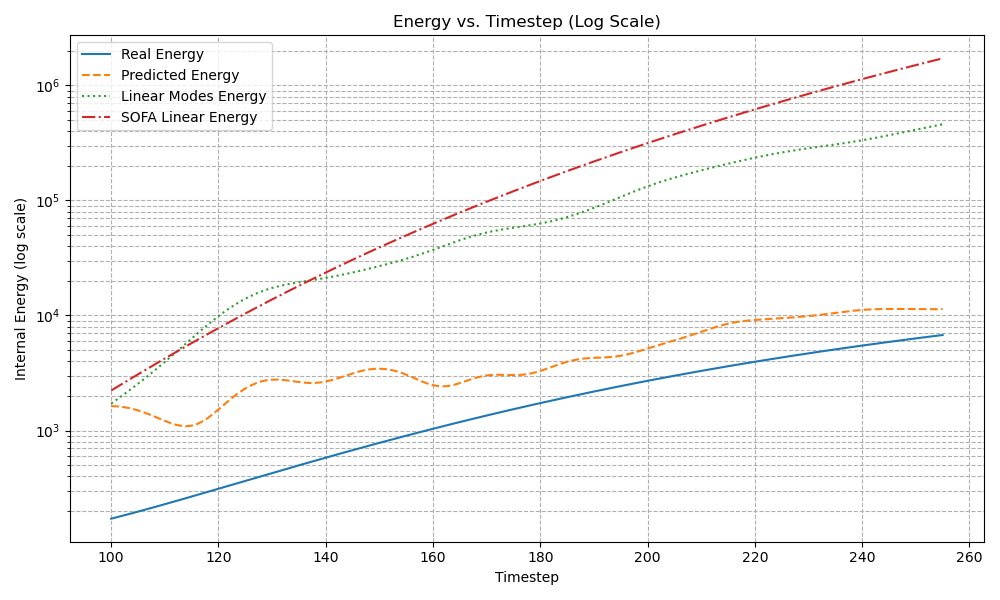
\includegraphics[width=0.45\textwidth]{Images/beam_dynamic_energy.png}
    \caption{Internal energy over time for dynamic cantilever beam simulation.}
    \label{fig:dynamic_validation_energy_comparison}
\end{figure}

This indicates that, despite limitations in long-term displacement prediction accuracy when trained solely on static data, the enhanced Neural Modes framework is able to predict a physically consistent energy evolution, which creates a more realistic simulation, albeit with some drift in displacement accuracy over time. 

\section{Conclusion and Future Work}
\label{sec:es:conclusion}

This thesis successfully enhanced the Neural Modes framework by adopting a supervised learning strategy with a physics-informed loss function. This modification effectively addressed limitations of the original self-supervised approach \cite{Wang_Du_Coros_Thomaszewski_2024}, particularly its performance in capturing large, nonlinear deformations. By training on a minimal dataset from full nonlinear FEM simulations, our enhanced framework demonstrated significantly improved accuracy in predicting displacement fields and better conservation of internal energy in the nonlinear regime, while maintaining the computational efficiency inherent in reduced-order models.

The numerical results on benchmark problems, such as the cantilever beam, clearly show the superior performance of the supervised Neural Modes model compared to traditional linear methods for large deformations. This indicates that the framework provides a promising approach for efficient and accurate simulation of hyperelastic materials.

Despite these advancements, a lot of room for future work remain. Improving the accuracy and stability of dynamic simulations over extended periods is crucial, potentially through more advanced temporal integration schemes or the integration of a fully reduced dynamic model.  

Overall, the enhanced Neural Modes framework represents a significant step towards bridging the gap between computational efficiency and simulation accuracy in nonlinear mechanics, highlighting the potential of physics-informed machine learning for real-time simulation applications in fields like biomedical engineering.


%---------------------------------------------------------------------------
%  BIBLIOGRAPHY
%---------------------------------------------------------------------------
% Remember to insert here only the essential bibliography of your work
\bibliography{bibliography.bib} % automatically inserted and ordered with this command 

\end{document}